
\documentclass[letterpaper,hide notes,xcolor={table,svgnames},10pt]{beamer}
\def\showexamples{t}


%\usepackage[svgnames]{xcolor}

%% Demo talk
%\documentclass[letterpaper,notes=show]{beamer}

\usecolortheme{crane}
\setbeamertemplate{navigation symbols}{}

\usetheme{MyPittsburgh}
%\usetheme{Frankfurt}

%\usepackage{tipa}

\usepackage{hyperref}
\usepackage{graphicx,xspace}
\usepackage[normalem]{ulem}
\usepackage{multicol}
\usepackage{amsmath,amssymb,amsthm,graphicx,xspace}
\newcommand\SF[1]{$\bigstar$\footnote{SF: #1}}

\usepackage[default]{sourcesanspro}
\usepackage[T1]{fontenc}
\usepackage[scaled]{beramono}
\usepackage{tikzpagenodes}

\newcounter{tmpnumSlide}
\newcounter{tmpnumNote}


% old question code
%\newcommand\question[1]{{$\bigstar$ \small \onlySlide{2}{#1}}}
% \newcommand\nquestion[1]{\ifdefined \presentationonly \textcircled{?} \fi \note{\par{\Large \textbf{?}} #1}}
% \newcommand\nanswer[1]{\note{\par{\Large \textbf{A}} #1}}


 \newcommand\mnote[1]{%
   \addtocounter{tmpnumSlide}{1}
   \ifdefined\showcues {~\tiny\fbox{\arabic{tmpnumSlide}}}\fi
   \note{\setlength{\parskip}{1ex}\addtocounter{tmpnumNote}{1}\textbf{\Large \arabic{tmpnumNote}:} {#1\par}}}

\newcommand\mmnote[1]{\note{\setlength{\parskip}{1ex}#1\par}}

%\newcommand\mnote[2][]{\ifdefined\handoutwithnotes {~\tiny\fbox{#1}}\fi
% \note{\setlength{\parskip}{1ex}\textbf{\Large #1:} #2\par}}

%\newcommand\mnote[2][]{{\tiny\fbox{#1}} \note{\setlength{\parskip}{1ex}\textbf{\Large #1:} #2\par}}

\newcommand\mquestion[2]{{~\color{red}\fbox{?}}\note{\setlength{\parskip}{1ex}\par{\Large \textbf{?}} #1} \note{\setlength{\parskip}{1ex}\par{\Large \textbf{A}} #2\par}\ifdefined \presentationonly \pause \fi}

\newcommand\blackboard[1]{%
\ifdefined   \showblackboard
  {#1}
  \else {\begin{center} \fbox{\colorbox{blue!30}{%
         \begin{minipage}{.95\linewidth}%
           \hspace{\stretch{1}} Some space intentionally left blank; done at the blackboard.%
         \end{minipage}}}\end{center}}%
         \fi%
}

\newcommand{\Rplus}{\protect\hspace{-.1em}\protect\raisebox{.35ex}{\small{\small\textbf{+}}}}
\newcommand{\CPP}{\mbox{C\Rplus\Rplus}\xspace}

%\newcommand\q{\tikz \node[thick,color=black,shape=circle]{?};}
%\newcommand\q{\ifdefined \presentationonly \textcircled{?} \fi}

\usepackage{listings,listings-rust}
\lstset{basicstyle=\footnotesize\ttfamily,
	breaklines=true,
	aboveskip=15pt,
  	belowskip=15pt,
	frame=lines,
	numbers=left, basicstyle=\scriptsize, numberstyle=\tiny, stepnumber=0, numbersep=2pt
}

\usepackage{siunitx}
\newcommand\sius[1]{\num[group-separator = {,}]{#1}\si{\micro\second}}
\newcommand\sims[1]{\num[group-separator = {,}]{#1}\si{\milli\second}}
\newcommand\sins[1]{\num[group-separator = {,}]{#1}\si{\nano\second}}
\sisetup{group-separator = {,}, group-digits = true}

%% -------------------- tikz --------------------
\usepackage{tikz}
\usetikzlibrary{positioning}
\usetikzlibrary{arrows,backgrounds,automata,decorations.shapes,decorations.pathmorphing,decorations.markings,decorations.text,decorations.pathreplacing}

\tikzstyle{place}=[circle,draw=blue!50,fill=blue!20,thick, inner sep=0pt,minimum size=6mm]
\tikzstyle{transition}=[rectangle,draw=black!50,fill=black!20,thick, inner sep=0pt,minimum size=4mm]

\tikzstyle{block}=[rectangle,draw=black, thick, inner sep=5pt]
\tikzstyle{bullet}=[circle,draw=black, fill=black, thin, inner sep=2pt]

\tikzstyle{pre}=[<-,shorten <=1pt,>=stealth',semithick]
\tikzstyle{post}=[->,shorten >=1pt,>=stealth',semithick]
\tikzstyle{bi}=[<->,shorten >=1pt,shorten <=1pt, >=stealth',semithick]

\tikzstyle{mut}=[-,>=stealth',semithick]

\tikzstyle{treereset}=[dashed,->, shorten >=1pt,>=stealth',thin]

\usepackage{ifmtarg}
\usepackage{xifthen}
\makeatletter
% new counter to now which frame it is within the sequence
\newcounter{multiframecounter}
% initialize buffer for previously used frame title
\gdef\lastframetitle{\textit{undefined}}
% new environment for a multi-frame
\newenvironment{multiframe}[1][]{%
\ifthenelse{\isempty{#1}}{%
% if no frame title was set via optional parameter,
% only increase sequence counter by 1
\addtocounter{multiframecounter}{1}%
}{%
% new frame title has been provided, thus
% reset sequence counter to 1 and buffer frame title for later use
\setcounter{multiframecounter}{1}%
\gdef\lastframetitle{#1}%
}%
% start conventional frame environment and
% automatically set frame title followed by sequence counter
\begin{frame}%
\frametitle{\lastframetitle~{\normalfont(\arabic{multiframecounter})}}%
}{%
\end{frame}%
}
\makeatother

\makeatletter
\newdimen\tu@tmpa%
\newdimen\ydiffl%
\newdimen\xdiffl%
\newcommand\ydiff[2]{%
    \coordinate (tmpnamea) at (#1);%
    \coordinate (tmpnameb) at (#2);%
    \pgfextracty{\tu@tmpa}{\pgfpointanchor{tmpnamea}{center}}%
    \pgfextracty{\ydiffl}{\pgfpointanchor{tmpnameb}{center}}%
    \advance\ydiffl by -\tu@tmpa%
}
\newcommand\xdiff[2]{%
    \coordinate (tmpnamea) at (#1);%
    \coordinate (tmpnameb) at (#2);%
    \pgfextractx{\tu@tmpa}{\pgfpointanchor{tmpnamea}{center}}%
    \pgfextractx{\xdiffl}{\pgfpointanchor{tmpnameb}{center}}%
    \advance\xdiffl by -\tu@tmpa%
}
\makeatother
\newcommand{\copyrightbox}[3][r]{%
\begin{tikzpicture}%
\node[inner sep=0pt,minimum size=2em](ciimage){#2};
\usefont{OT1}{phv}{n}{n}\fontsize{4}{4}\selectfont
\ydiff{ciimage.south}{ciimage.north}
\xdiff{ciimage.west}{ciimage.east}
\ifthenelse{\equal{#1}{r}}{%
\node[inner sep=0pt,right=1ex of ciimage.south east,anchor=north west,rotate=90]%
{\raggedleft\color{black!50}\parbox{\the\ydiffl}{\raggedright{}#3}};%
}{%
\ifthenelse{\equal{#1}{l}}{%
\node[inner sep=0pt,right=1ex of ciimage.south west,anchor=south west,rotate=90]%
{\raggedleft\color{black!50}\parbox{\the\ydiffl}{\raggedright{}#3}};%
}{%
\node[inner sep=0pt,below=1ex of ciimage.south west,anchor=north west]%
{\raggedleft\color{black!50}\parbox{\the\xdiffl}{\raggedright{}#3}};%
}
}
\end{tikzpicture}
}


%% --------------------

%\usepackage[excludeor]{everyhook}
%\PushPreHook{par}{\setbox0=\lastbox\llap{MUH}}\box0}

%\vspace*{\stretch{1}

%\setbox0=\lastbox \llap{\textbullet\enskip}\box0}

\setlength{\parskip}{\fill}

\newcommand\noskips{\setlength{\parskip}{1ex}}
\newcommand\doskips{\setlength{\parskip}{\fill}}

\newcommand\xx{\par\vspace*{\stretch{1}}\par}
\newcommand\xxs{\par\vspace*{2ex}\par}
\newcommand\tuple[1]{\langle #1 \rangle}
\newcommand\code[1]{{\sf \footnotesize #1}}
\newcommand\ex[1]{\uline{Example:} \ifdefined \presentationonly \pause \fi
  \ifdefined\showexamples#1\xspace\else{\uline{\hspace*{2cm}}}\fi}

\newcommand\ceil[1]{\lceil #1 \rceil}


\AtBeginSection[]
{
   \begin{frame}
       \frametitle{Outline}
       \tableofcontents[currentsection]
   \end{frame}
}



\pgfdeclarelayer{edgelayer}
\pgfdeclarelayer{nodelayer}
\pgfsetlayers{edgelayer,nodelayer,main}

\tikzstyle{none}=[inner sep=0pt]
\tikzstyle{rn}=[circle,fill=Red,draw=Black,line width=0.8 pt]
\tikzstyle{gn}=[circle,fill=Lime,draw=Black,line width=0.8 pt]
\tikzstyle{yn}=[circle,fill=Yellow,draw=Black,line width=0.8 pt]
\tikzstyle{empty}=[circle,fill=White,draw=Black]
\tikzstyle{bw} = [rectangle, draw, fill=blue!20, 
    text width=4em, text centered, rounded corners, minimum height=2em]
    
    \newcommand{\CcNote}[1]{% longname
	This work is licensed under the \textit{Creative Commons #1 3.0 License}.%
}
\newcommand{\CcImageBy}[1]{%
	\includegraphics[scale=#1]{creative_commons/cc_by_30.pdf}%
}
\newcommand{\CcImageSa}[1]{%
	\includegraphics[scale=#1]{creative_commons/cc_sa_30.pdf}%
}
\newcommand{\CcImageNc}[1]{%
	\includegraphics[scale=#1]{creative_commons/cc_nc_30.pdf}%
}
\newcommand{\CcGroupBySa}[2]{% zoom, gap
	\CcImageBy{#1}\hspace*{#2}\CcImageNc{#1}\hspace*{#2}\CcImageSa{#1}%
}
\newcommand{\CcLongnameByNcSa}{Attribution-NonCommercial-ShareAlike}

\newenvironment{changemargin}[1]{% 
  \begin{list}{}{% 
    \setlength{\topsep}{0pt}% 
    \setlength{\leftmargin}{#1}% 
    \setlength{\rightmargin}{1em}
    \setlength{\listparindent}{\parindent}% 
    \setlength{\itemindent}{\parindent}% 
    \setlength{\parsep}{\parskip}% 
  }% 
  \item[]}{\end{list}} 




\title{Lecture 31 --- Introduction to Queueing Theory}

\author{Jeff Zarnett\\ \small \texttt{jzarnett@uwaterloo.ca}}
\institute{Department of Electrical and Computer Engineering \\
  University of Waterloo}
\date{\today}


\begin{document}

\begin{frame}
  \titlepage

 \end{frame}



\begin{frame}
\frametitle{Queueing Theory}

Literally the theory of queues -- what makes queues appear, how will they behave, and how do we make them go away? 


Queueing theory has played a role in your life whether you know it or not. 



\end{frame}

\begin{frame}
\frametitle{Queueing Theory}

This is how tech support at Rogers or Bell or Telus or whomever decides just how many customer service agents to have available at any given time. 

\begin{center}
	
\includegraphics[width=0.5\textwidth]{images/techsupport.jpg}
\end{center}

Queueing theory is applicable to lots of fields, including industrial design, call centres, telecom systems, and computers executing transactions. 

\end{frame}



\begin{frame}
\frametitle{Questions Queueing Theory Helps Answer}

\begin{itemize}
 \item Given a choice between a single machine with speed $s$ or $n$ machines, each with speed $s/n$, which should we choose?
 \item If the arrival rate and service rate double, how does the mean response time change?
 \item Should we try to balance load or is that a waste of time/effort?
 \item Can we give priority to certain operations without harming another category of job?
 \item How do job size variability and heavy-tailed workloads affect our choices of scheduling policy?
 \item If 12 servers is enough to handle 9 jobs per second, do we need 12~000 servers if we have an arrival rate if 9~000 jobs per second?
\end{itemize}

\end{frame}



\begin{frame}
\frametitle{Formal Terms and Bank Analogies}

\begin{itemize}
	\item Server - The banking centre fulfilling customer requests.
	\item Customer - Initiator of service requests.
	\item Wait time - The time a customer spends waiting in line.
	\item Service time - The time from when a teller starts to serve a customer up to the time when the next customer is called forward.
	\item Arrival rate - The rate at which customers arrive.
	\item Service rate - the rate at which customer requests are serviced.

\end{itemize}

\end{frame}



\begin{frame}
\frametitle{Formal Terms and Bank Analogies}

\begin{itemize}
	\item Utilization - The fraction of the teller's time used actually handling customer requests (not idling).
	\item Queue length - The total number of customers waiting, or currently with a teller, or both.
	\item Response time - The sum of wait and service time for a single visit.
	\item Residence time - The total response time if a customer visits several tellers (or the same one multiple times).
	\item Throughput - The rate at which customers get their requests serviced and dealt with.
\end{itemize}

\end{frame}



\begin{frame}
\frametitle{Mathematical Symbol Table}

\begin{center}
	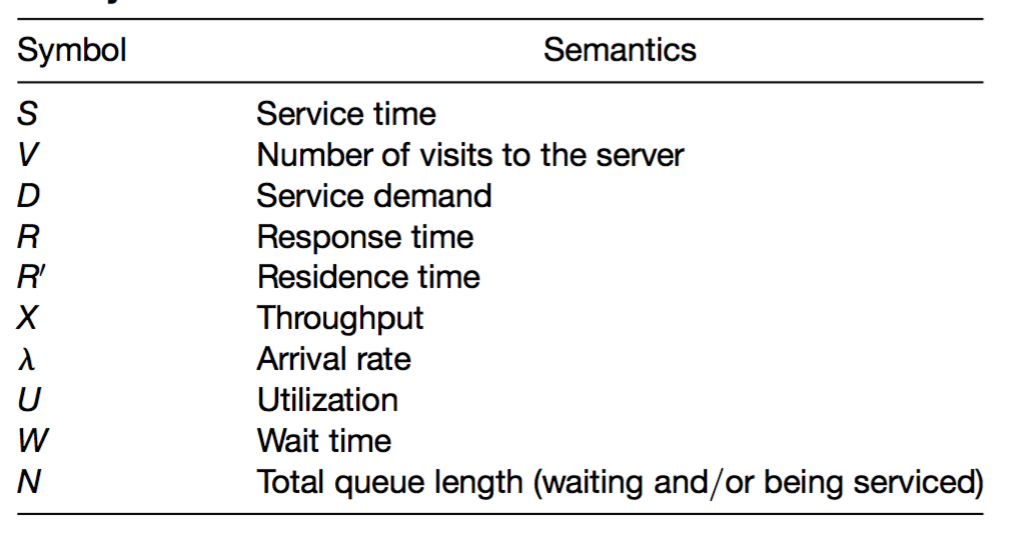
\includegraphics[width=0.85\textwidth]{images/math-symbols.png}
\end{center}

\end{frame}



\begin{frame}
\frametitle{Trade-Offs}

It's actually (allegedly) a trade-off: if I have to wait too long to do my banking, I could always take my business elsewhere. 

Minimizing customer wait time makes customers happy, so that's something the bank should want. 

It would also be nice if the bank trains its tellers well, so they can complete all operations, even unusual ones, quickly and efficiently, reducing service time.

Overstaffed is bad and understaffed is also bad. 

\end{frame}


\begin{frame}
\frametitle{Pizza has priority}

\begin{center}
	
\includegraphics[width=0.5\textwidth]{images/dmv.png}
\end{center}

\end{frame}



\begin{frame}
\frametitle{Computer World}

Back to the realm of computers: you have lots of queues in your computer. 

The CPU uses a time-sharing scheduler to run as many concurrent programs as possible. 

A router has a queue for packets (data) that has a maximum size, and if this is exceeded, packets will be simply dropped. 

Queueing theory gives us a formal framework with which to grapple with our problems instead of just guessing.


\end{frame}



\begin{frame}
\frametitle{Simple Example}

Imagine we have a system with one CPU that serves a queue of jobs in First-Come-First-Served (FCFS) order with an arrival rate $\lambda$ of 3 jobs per second. 

Each job takes some amount of time and resources. 

Suppose the average service rate $\mu$ is 5 jobs per second. 

The system is not overloaded -- 3 jobs per second arriving is less than 5 jobs per second being serviced. 

\end{frame}



\begin{frame}
\frametitle{Scale Up}

Suppose now that your boss says that tomorrow the arrival rate will double.

If you do nothing: 6 jobs arriving per second, on average, to a system that can service, on average, 5 jobs per second. 

You have been allocated some budget to replace the CPU with a faster one.

\end{frame}



\begin{frame}
\frametitle{Simple Example Scaling}

\begin{center}
	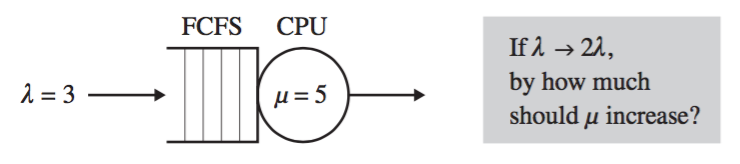
\includegraphics[width=0.7\textwidth]{images/qt-example1.png}
\end{center}

Goal: Customers should not notice the increase in arrival rate. 

So, should we (1) double the CPU speed; (2) more than double the CPU speed; or (3) less than double the CPU speed?

\end{frame}



\begin{frame}
\frametitle{Option 3}


The answer is (3) - we don't need to double the CPU speed. 

We can see later in formal terms why this is the case, but think for a minute about what it is? 

If we double the service rate and double the arrival rate, we actually get half the mean response time...


\end{frame}



\begin{frame}
\frametitle{Alternate Scenario}

There are always $N=6$ jobs running at a time. 

As soon as a job completes, a new one is started (this is called a \alert{closed system}). 

Each job goes through to be processed on one of two servers, each of which has a service time $\mu$ of 1 job per 3 seconds.

\end{frame}



\begin{frame}
\frametitle{Closed System}

\begin{center}
	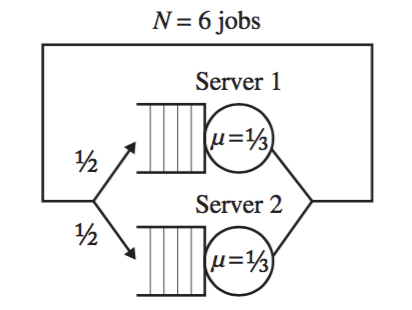
\includegraphics[width=0.5\textwidth]{images/qt-example2.png}
\end{center}

\end{frame}



\begin{frame}
\frametitle{Only Trying to Help...}

Bad news: sometimes, improvements do nothing. 

If we replace server 1 with one which is $2\times$ faster (so 2 jobs per 3 seconds), does that help? \emph{Nope. Not really.}

Does raising $N$ help? \emph{Nope, negligible effect.}

Strangely, dropping $N$ to 1 means the server replacement makes a difference, if you can call that improvement.

\end{frame}



\begin{frame}
\frametitle{Open It Up}

What if it's an \alert{open system} where arrival times are independent of completion?

\begin{center}
	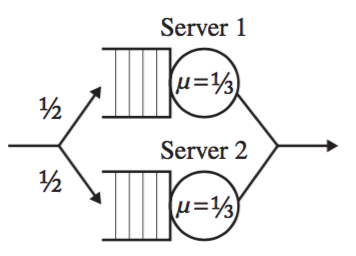
\includegraphics[width=0.5\textwidth]{images/qt-example2-2.png}
\end{center}

In this case, yes, replacing server 1 makes a huge difference!

\end{frame}



\begin{frame}
\frametitle{One Fast Server, or $n$ Slow Ones?}

Do we want one fast server or $n$ slower ones? 

What is better if we want to minimize the mean response time when we have non-preemptable jobs?

\begin{center}
	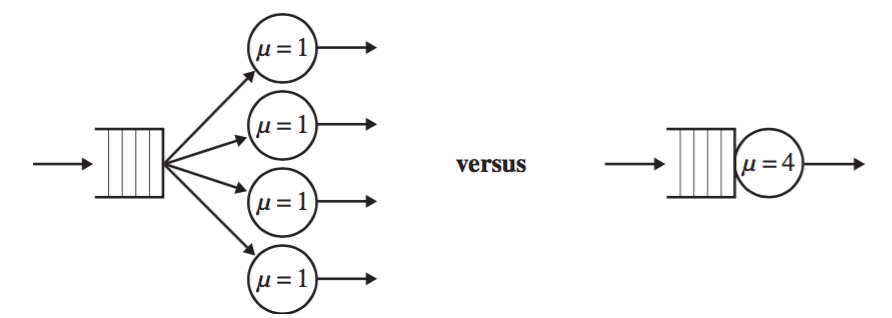
\includegraphics[width=0.9\textwidth]{images/qt-example3.png}
\end{center}

\end{frame}



\begin{frame}
\frametitle{Answer: It Depends}

One big factor is the variability of the job sizes. 

Imagine you are at the grocery store and most people have 12 items or fewer and there's one guy who's buying 85 items. 

You don't want to be standing in line with milk and eggs behind someone who is trying to buy six of everything, do you? 

So if there's high variability, you probably want multiple servers.

\end{frame}



\begin{frame}
\frametitle{Alternatives}

What if the load is low? 

Chances are you would prefer the one fast server instead of having some number of servers doing nothing.

What if jobs are interruptible (preemptible)? 

You could always use a single fast machine to simulate $n$ slow machines, so a single fast machine is at least as good as the alternative. 

\end{frame}



\begin{frame}
\frametitle{Digression on Load Balancing}

Imagine your typical ``server farm'' - you have $n$ servers that are all responsible for handling incoming requests. 

Let's imagine all servers are the same (or close enough). 

What we typically see in load balancing is assignment of tasks to servers via some dispatcher:

\begin{center}
	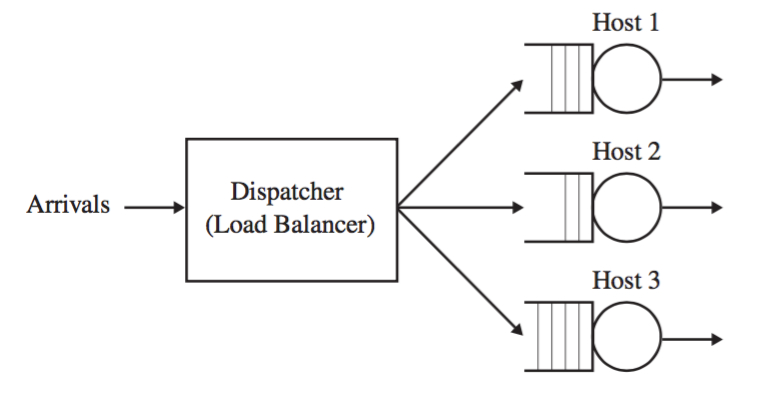
\includegraphics[width=0.6\textwidth]{images/central-dispatcher.png}
\end{center}

\end{frame}



\begin{frame}
\frametitle{Assignment Policies}

There are a few different task assignment policies - ways in which we can assign work to servers:

\begin{itemize}
	\item Random
	\item Round-Robin
	\item Shortest-Queue
	\item Size-Interval-Task-Assignment
	\item Least-Work-Left
	\item Central-Queue
\end{itemize}

\end{frame}


\begin{frame}
\frametitle{Red Line Overload}

\begin{center}
	
\includegraphics[width=0.8\textwidth]{images/topgun.jpg}
\end{center}

``You'll never say hello to you\\
Until you get it on the red line overload\\
You'll never know what you can do\\
Until you get it up as high as you can go''
 
\hfill - Kenny Loggins


\end{frame}



\begin{frame}
\frametitle{Red Line Overload}

Earlier I mentioned it would probably be bad to see 6 jobs arriving per second to a system that can handle 5 per second. 

This doesn't seem like rocket science, but it bears repeating. 

In our discussion we require that $\lambda \leq \mu$ and assume that $\lambda < \mu$. 

That is to say, we are not overloaded.

\end{frame}



\begin{frame}
\frametitle{Red Line Overload}

Remember now that the values for $\lambda$ and $\mu$ are averages. 

It could happen that temporarily we ``fall behind'' a bit, but then make up for it a little later on... 

Think about the long term, though---if we are not at least keeping up then this will eventually get out of hand. 

How badly? Well, in the limit, the queue length goes to infinity.

\end{frame}



\begin{frame}
\frametitle{The Proof is the Proof}

Let's represent time with $t$ and define $N(t)$ as the number of jobs in the system at time $t$.

$A(t)$ represents arrivals by time $t$ and $D(t)$ represents departures by time $t$.

\begin{center}
	$E[N(t)] = E[A(t)] - E[D(t)] \geq \lambda t - \mu t = t (\lambda - \mu) $
\end{center}

If arrivals exceed departures  $t (\lambda - \mu) $ also goes to infinity.

\end{frame}



\begin{frame}
\frametitle{Raise the Throughput}

Raising $\mu$ is generally desirable. 

This is, after all, programming for performance---the faster we complete work, the more work we can get done in the same amount of time. 

Improving the service rate, however, does not necessarily improve the throughput. 

\end{frame}



\begin{frame}
\frametitle{Wait, What?}

We've assumed that the arrival rate is less than the service rate. 

So we have enough capacity to handle all incoming work. 

So the limiting factor on completed work is actually arriving work. 

We have the capacity to do at least what is arriving and possibly a bit more. 

Adding more work capacity doesn't mean more work gets done if there isn't any more work to do.

So raising $\mu$ increases the maximum possible throughput, but does not necessarily increase the actual throughput.

\end{frame}



\begin{frame}
\frametitle{But Closed Systems...}


In a closed system: one in which there is always more work to do and as soon as one item is finished the next one enters the queue. 

 In that case, we are running at capacity all the time, so actually $\mu$ is the controlling factor -- the throughput is exactly the service rate. 
 
 \begin{center}
	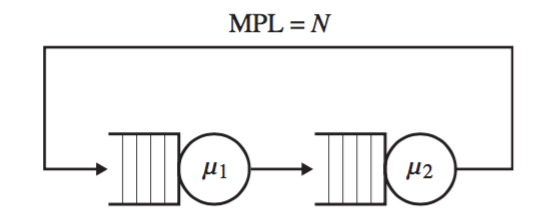
\includegraphics[width=0.4\textwidth]{images/tandem-closed.png}
\end{center}

What is the throughput here?  Intuition suggests min($\mu_{1}, \mu_{2}$), right? 

\end{frame}



\begin{frame}
\frametitle{Throughput in the Closed System}



Sometimes. This is okay if the slower server is always busy, but that's not always the case. 

What if $N$ is 1? Okay, that's a bit of an exception case though. 

What about $N$ being 2? Then the slower server has some work to do at all times right?

\end{frame}



\begin{frame}
\frametitle{Throughput in the Closed Systems}

Nope, sadly not. 

Sometimes the slow server is faster than the fast server, because $\mu_{1}$ and $\mu_{2}$ are just averages. 

And averages can be misleading! 

The average family might have 2.3 children (or whatever the figure is), but you can't exactly have 0.3 of a child...

\end{frame}



\begin{frame}
\frametitle{Don't Guess...}
Some smart folks at IBM wanted to know, given the arrival rate $\lambda$, what was the mean job size, $E[S]$ (which is $1/\mu$). 

Our experiment should be a hundred runs of sending a single job into the system and averaging the values. 

This is okay, but does not reflect reality where we have things like caching of data and multiple concurrent jobs. 

\end{frame}



\begin{frame}
\frametitle{Don't Guess...}

The open system strategy is: ramp up $\lambda$. 

Keep piling more jobs on the system. 

At some point the system will not be able to keep up. Once the completion rate levels off, we hit the limit and we have a value for $\mu$.


\end{frame}



\begin{frame}
\frametitle{Don't Guess...}

The closed system strategy: set it up so there is always work to do. 

In closed systems, there's often consideration given to \textit{think time} -- this is what happens when the user is on the command line and dispatching work to do. 

To keep the system totally busy in the stress test, we need think time to be zero---so additional work is always available. 

And then we can simply measure the jobs completing per second, giving us $\mu$ directly.


\end{frame}



\end{document}

